\documentclass[border=10pt]{standalone}
\usepackage{tikz}
\begin{document}
% A rotated node's own anchors rotate with it, and `anchor=` names one of those ROTATED anchors to
% sit on the point. Filling the node prices where its ink lands; the dot at (0,0) is the point itself.
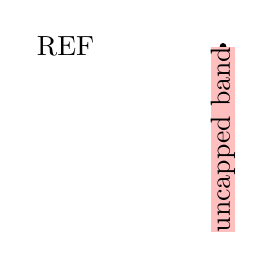
\begin{tikzpicture}[x=1cm,y=1cm]
  \node (A) at (-2,0) {REF};
  \fill (0,0) circle (1.2pt);
  \node[anchor=east,rotate=90,fill=red!25,inner sep=0pt] at (0,0) {uncapped band};
\end{tikzpicture}
\end{document}
